\section{Theorie}
\label{sec:Theorie}
Ionenkristalle, wie beispielsweise Kaliumbromid (KBr), bestehen aus Kationen (K$^{+}$) und Anionen (Br$^{-}$), welche
auf festen Gitterplätzen angeordnet sind.
Wird eine Störstelle wie ein zweiwertiges Kation, zum Beispiel Sr$^{2+}$, in den Kristall eingebaut so
entsteht eine Leerstelle an einer anderen Kationen-Stelle um die lokale Ladungsneutralität aufrecht zu erhalten.
So entsteht ein elektrischer Dipol mit Richtung entlang der Achse der Störstellen. Dies ist in \autoref{fig:Störstelle}
beispielsweise für einen Cäsiumjodid Kristall dargestellt.
\begin{figure}[H]
  \centering
  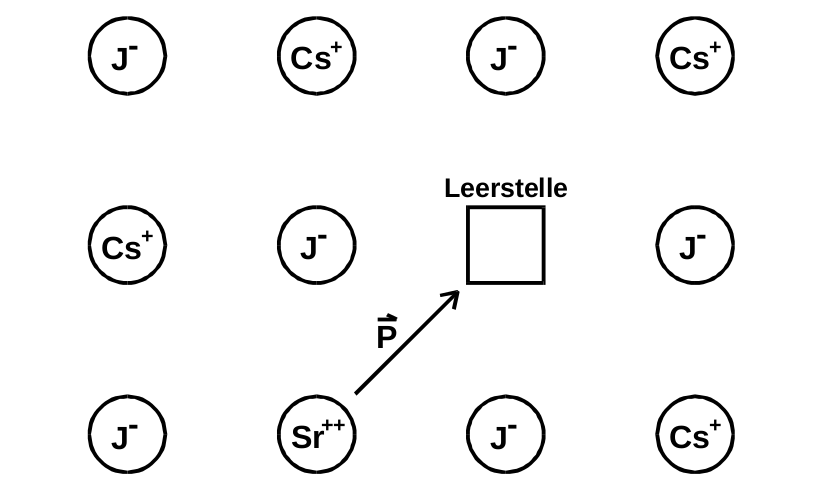
\includegraphics[width=0.6\textwidth]{pics/Stoerstelle.png}
  \caption{Schematische Darstellung eines Ionenkristalls mit einem, durch
  zwei Störstellen erzeugten, elektrischen Dipol \cite{Anleitung}.}
  \label{fig:Störstelle}
\end{figure}
Die Orientierung der Dipole sind statistisch im Raum verteilt, jedoch sind dabei auf Grund der Gitterstruktur
nur diskrete Richtungen und Beträge möglich. Eine Änderung der Richtung
kann unter einer Temperatur von 500 K nur durch Leerstellendiffusion erfolgen.
Dazu wird eine bestimmte, materialspezifische Energie $W$ benötigt, um das Gitterpotential zu überwinden.
Die Anzahl der Dipole mit einer ausreichend großen thermischen Energie folgt der Boltzmann-Statistik.
Ebenso folgt die mittlere Zeit zwischen zwei Umorientierungen, die Relaxationszeit $\tau$, dieser Verteilung.
\begin{equation}
  \tau(T) = \tau_0 \exp{\left(\frac{W}{kT}\right)}
  \label{eq:Relaxationszeit}
\end{equation}
Dabei ist $\tau_0$ die charakteristische Relaxationszeit.\\
Wird der Kristall in ein elektrisches Feld gebracht richtet sich ein Teil $y$ der Dipole in Richtung
des Feldes aus. Dieser wird durch die Langevin-Funktion
\begin{equation}
  y = L\left( \frac{pE}{kT}\right) = \coth{\left( \frac{pE}{kT}\right) - \frac{kT}{pE}}
  \label{eq:Lagevin}
\end{equation}
beschrieben, welche für $pE \ll kT$ mit
\begin{equation}
  y(T)=\frac{pE}{3kT}
  \label{eq:LagevinNäherung}
\end{equation}
genähert werden kann.
Da die Relaxation thermisch bedingt ist, lässt sich die Ausrichtung bei tiefen Temperaturen
einfrieren.
Da \autoref{eq:Relaxationszeit} Temperaturabhängig ist, richten sich die Dipole bei zunehmender Temperatur
wieder nach einer statistischen Verteilung aus. Dies erzeugt einen Depolarisationsstrom, falls
die bewegten Ladungsträger im Ionenkristall entfernt wurden.
Die Stromdichte
\begin{equation}
  j(T)=y\left(T_{\symup{p}}\right)\,p\,\frac{\symup{d}{N}}{\symup{d}{t}}
\label{eq:Stromdichte}
\end{equation}
setzt sich aus der Anzahl der vorher ausgerichteten Dipole $y\left(T_{\symup{p}}\right)$ ,
dem Dipolmoment $p$ und der Rate der relaxierenden Dipole $\frac{\symup{d}{N}}{\symup{d}{t}}$
zusammen. Dies lässt sich mit \autoref{eq:LagevinNäherung} als
\begin{equation}
  j(T)=\frac{p^2 E}{3kT_{\symup{p}}}\frac{\symup{d}{N}}{\symup{d}{t}}
  \label{eq:StromdichteNäherung1}
\end{equation}
schreiben.
Die Zahl der pro Zeitintervall relaxierenden Dipole ist proportional zur Zahl
der noch orientierten Dipole und antiproportional zur Relaxationszeit $\tau(T)$.
Dies lässt sich unter der Berücksichtigung einer konstanten Heizrate $b \tau_0$ durch
\begin{equation}
  j(T) = \frac{p^2E}{3kT_p}\frac{N_p}{\tau_0}\exp{\left(-\frac{1}{}\int^T_{T_0}\exp{\left(-\frac{W}{kT'}\right)}\symup{d}T'\right)}\exp{\left(-\frac{W}{kT}\right)}.
  \label{eq:StromdichteIntegral}
\end{equation}
ausdrücken, was sich durch
\begin{equation}
    j(T)=\frac{p^2 E}{3kT_{\symup{p}}}\frac{N_{\symup{p}}}{\tau_0}\exp{\left(\frac{-W}{kT}\right)}
\label{eq:StromdichteNäherung2}
\end{equation}
nähern lässt.\\
\\Für den Verlauf der Kurve des Depolarisationsstrom in Abhängigkeit der Temperatur wird ein steiler Anstieg,
ein Maximum und danach wieder ein Abfallen des Stroms erwartet.
Da der Strom durch den Abfall von $\tau(T)$ mit steigender Temperatur zunächst zunimmt
und die Relaxationsrate stetig fällt. Es kann ein zweites Maximum auftreten, welches durch weitere Relaxationen mit höherem $W$ hervorgerufen wird.\\
\\Ohne das Integral zu nähern lässt sich $\tau(T)$ durch Integration des Stromes nach
\begin{equation}
  \tau(T) = \frac{\int_{T}^{\infty}i(T')\symup{d}T'}{bi(T)}
  \label{eq:tau2}
\end{equation}
berechnen.
Aus einem gemessenen Verlauf $i(T)$ lässt sich somit $W$ durch die Steigung einer linearen Ausgleichsgeraden an die logarithmierten Verläufe von \eqref{eq:tau2}, bzw. \eqref{eq:StromdichteNäherung2}, bestimmen.
Zur Bestimmung von $\tau_0$ betrachtet man die Lage des Maximums von $i(T)$. Dieses liegt nach \eqref{eq:StromdichteNäherung2} bei
\begin{equation}
  \tau_{max}(T) = \frac{HkT_{max}^2}{W}.
  \label{eqn:tau3}
\end{equation}
Mit Hilfe dieses Wertes und \eqref{eq:Relaxationszeit} lässt sich nun $\tau_0$ berechnen.
